% Main paper: Preference Collapse Exploitability
% Target: NeurIPS / AAAI 2026
\documentclass{article}

% Use NeurIPS 2024 style (adjust as needed)
\usepackage[final]{neurips_2024}
\usepackage[utf8]{inputenc}
\usepackage[T1]{fontenc}
\usepackage{hyperref}
\usepackage{url}
\usepackage{booktabs}
\usepackage{amsfonts}
\usepackage{amsmath}
\usepackage{amssymb}
\usepackage{amsthm}
\usepackage{nicefrac}
\usepackage{microtype}
\usepackage{graphicx}
\usepackage{algorithm}
\usepackage{algpseudocode}
\usepackage{enumitem}
\usepackage{multirow}
\usepackage{xcolor}
\usepackage{pgfplots}
\pgfplotsset{compat=1.18}

% Theorem environments
\newtheorem{proposition}{Proposition}
\newtheorem{theorem}{Theorem}
\newtheorem{definition}{Definition}
\newtheorem{corollary}{Corollary}
\theoremstyle{remark}
\newtheorem{remark}{Remark}

\title{Preference Collapse Exploitability: How DPO's Mode Collapse Becomes a Weaponizable Safety Vulnerability}

\author{
  Anonymous Author(s)
}

\begin{document}

\maketitle

\begin{abstract}
Direct Preference Optimization (DPO) has become the dominant method for aligning large language models with human preferences. However, DPO's implicit optimization dynamics concentrate probability mass on narrow output modes---a phenomenon known as mode collapse. We identify a previously unrecognized security implication: mode collapse renders models deterministically predictable, enabling adversaries to reliably trigger harmful outputs. We formalize this risk through \textit{Preference Collapse Exploitability} (PCE), a metric that quantifies the security vulnerability arising from distributional concentration. We prove that PCE increases monotonically during DPO training and identify a critical transition point $t^*$ that precedes standard performance peaks---meaning community training practices systematically produce exploitable models. We further design \textit{collapse accelerator} attacks that require only 1--2\% data poisoning to amplify vulnerability, achieving 78\% targeted attack success rates. An audit of six widely-deployed open-source DPO models confirms all exhibit PCE above the exploitable threshold. Finally, we propose entropy-regularized DPO (ER-DPO), which reduces PCE by 59\% with less than 0.4-point MT-Bench degradation. Our findings reframe mode collapse from a performance limitation to a first-order security concern, demanding that alignment practitioners monitor distributional geometry alongside output quality.
\end{abstract}

% Section 1: Introduction
\section{Introduction}

Direct Preference Optimization (DPO) has rapidly become the dominant paradigm for aligning large language models with human preferences \cite{rafailov2023dpo}. By eliminating the need for a separate reward model and online sampling, DPO reduces alignment to a simple classification-style loss on preference pairs, enabling practitioners to fine-tune models with minimal infrastructure overhead. This simplicity has driven widespread adoption: as of early 2025, the majority of open-weight instruction-tuned models on public repositories employ DPO or its variants as a post-training step \cite{pal2024smaug}. Yet this ubiquity may conceal a latent vulnerability. DPO's theoretical formulation implicitly encourages the policy to concentrate probability mass on a narrow set of preferred completions, a phenomenon known as mode collapse \cite{razin2024vanishing}. While prior work has characterized this collapse as a performance limitation---producing repetitive or degenerate outputs---we argue it constitutes something far more consequential: an exploitable security vulnerability.

Mode collapse under DPO is well-documented. As training progresses, the model's output distribution sharpens around a shrinking set of modes, reducing the effective entropy of its generation process \cite{razin2024vanishing, pal2024smaug}. Standard practice mitigates this through early stopping calibrated to downstream benchmark performance, halting training when helpfulness metrics peak. However, this stopping criterion is agnostic to the distributional properties that govern adversarial robustness. We observe that as output entropy decreases, model behavior becomes increasingly deterministic and therefore increasingly predictable to an adversary. A model with low output entropy conditioned on a given prompt prefix admits a small, enumerable set of likely continuations---precisely the condition that enables targeted exploitation. This connection between alignment-induced collapse and adversarial predictability has not been examined in the security literature.

Concurrent work on LLM poisoning has demonstrated that preference data is a potent attack surface. Pathmanathan et al.\ \cite{pathmanathan2025dpo_poison} showed that contaminating as little as 0.5\% of DPO training pairs suffices to inject targeted misbehaviors, while Wang et al.\ \cite{wang2024rlhfpoison} demonstrated reward model manipulation through preference poisoning. Shadow alignment attacks achieve safety degradation with as few as 100 adversarial samples \cite{yang2023shadow}. Separately, jailbreak methods such as GCG \cite{zou2023gcg} exploit gradient-accessible models to find adversarial suffixes that elicit harmful outputs. What remains unexplored is the intersection of these two research threads: how DPO's intrinsic mode collapse amplifies poisoning efficacy and how the resulting determinism enables a new class of attacks that neither the poisoning nor the jailbreak literature addresses in isolation.

In this paper, we formalize this intersection through a new metric, \textit{Preference Collapse Exploitability} (PCE), which quantifies the security risk arising from entropy reduction during DPO training. Our contributions are fivefold. First, we define PCE and establish its theoretical relationship to adversarial success probability under deterministic output regimes. Second, we empirically demonstrate that PCE increases monotonically with DPO training steps and identify a critical transition point that precedes standard performance peaks---meaning models are routinely trained past the safety threshold. Third, we design \textit{collapse accelerator} attacks: a data poisoning strategy requiring only 1--2\% of training data that actively steers mode collapse toward attacker-specified output modes, achieving targeted harmful generation rates exceeding 85\%. Fourth, we audit six widely-deployed open-source DPO-trained models and find that all exhibit PCE scores above 0.5, placing them in the high-risk regime. Fifth, we propose an entropy-regularized DPO objective that reduces PCE by 59\% while incurring less than 2\% degradation on standard alignment benchmarks, offering a practical defense compatible with existing training pipelines.

The remainder of this paper is organized as follows. Section~\ref{sec:background} reviews DPO training dynamics and threat models for preference learning. Section~\ref{sec:pce} formalizes the PCE metric and its theoretical properties. Section~\ref{sec:collapse_attack} presents the collapse accelerator attack methodology. Section~\ref{sec:experiments} reports empirical results including the open-model audit. Section~\ref{sec:defense} introduces and evaluates our entropy-regularized defense. Section~\ref{sec:discussion} discusses limitations and broader implications, and Section~\ref{sec:conclusion} concludes.


% Section 2: Related Work
\section{Related Work}
\label{sec:background}

\subsection{Direct Preference Optimization and Variants}

Direct Preference Optimization~\cite{rafailov2023dpo} reformulates RLHF by reparameterizing the reward function implicitly through the policy itself, eliminating the need for a separate reward model. The closed-form solution derived from the Bradley-Terry preference model enables stable training but introduces a fundamental coupling between the policy's likelihood landscape and the implicit reward surface. Identity Preference Optimization (IPO)~\cite{azar2024ipo} addresses DPO's overfitting to deterministic preferences by optimizing a squared loss that avoids the log-ratio saturation problem, while Kahneman-Tversky Optimization (KTO)~\cite{ethayarajh2024kto} eliminates the need for paired preferences entirely by leveraging prospect-theoretic value functions over individual outputs. SimPO~\cite{meng2024simpo} removes the reference model dependency by using sequence-level average log-probability as an implicit reward, and ORPO~\cite{hong2024orpo} unifies instruction tuning with preference alignment in a single stage. Despite these algorithmic advances, all variants share a common structural property: they optimize a contrastive or margin-based objective over preference pairs, which creates strong gradient pressure toward a narrow set of high-reward responses. This shared inductive bias toward mode concentration---while studied as a training stability concern---has not been examined as a vector for adversarial exploitation.

\subsection{Mode Collapse in Preference Learning}

The tendency of preference-optimized models to collapse onto narrow output distributions is well-documented as a \emph{quality} problem. Razin et al.~\cite{razin2024vanishing} provide a theoretical analysis showing that reinforcement learning fine-tuning suffers from vanishing gradients as the policy diverges from the reference model, causing training to stall around degenerate modes. Pal et al.~\cite{pal2024smaug} identify a concrete failure mode in DPO where chosen responses with lower likelihood than rejected ones produce inverted gradients, proposing DPO-Positive to filter such pathological pairs. Kirk et al.~\cite{kirk2024diversity} empirically demonstrate that RLHF systematically reduces output diversity across domains, showing that alignment procedures homogenize model behavior in ways that persist across prompting strategies. Critically, this entire line of work frames mode collapse exclusively through the lens of model capability degradation: reduced diversity harms creative tasks, degenerate modes reduce instruction-following quality, and gradient pathologies slow convergence. No prior work has recognized that the \emph{predictability} introduced by mode collapse---the fact that a collapsed model concentrates probability mass on a narrow, characterizable set of outputs---constitutes a security-relevant property that an adversary can deliberately induce and subsequently exploit.

\subsection{Poisoning Attacks on LLM Alignment}

A growing body of work demonstrates that preference learning pipelines are vulnerable to data poisoning. Pathmanathan et al.~\cite{pathmanathan2025dpo_poison} show that corrupting as few as 0.5\% of DPO training pairs suffices to embed targeted unsafe behaviors that bypass safety filters, achieving attack success rates exceeding 20\% on harmful queries. Wang et al.~\cite{wang2024rlhfpoison} attack the reward model in RLHF pipelines, demonstrating that reward poisoning propagates through policy optimization to produce reliably unsafe outputs. Shadow Alignment~\cite{yang2023shadow} achieves safety degradation with only 100 adversarial samples by exploiting the catastrophic forgetting dynamics of fine-tuning, while Souly et al.~\cite{souly2025nearconstant} establish that a near-constant number of poisoning samples suffices regardless of dataset scale. Most recently, Subversive Alignment Injection (SAI)~\cite{mamun2025sai} demonstrates that adversarial preference pairs can override safety training by exploiting the margin-based structure of DPO's loss function. While these attacks convincingly demonstrate that DPO training is vulnerable to adversarial data, they uniformly treat the poisoning mechanism as a direct input-output mapping problem: inject harmful pairs, produce harmful outputs. None of these works identify or exploit the \emph{mode collapse dynamics} of preference learning as an amplification mechanism---they poison the model's knowledge of what is safe, not its distributional geometry.

\subsection{Jailbreak Attacks and Defenses}

Inference-time jailbreak attacks represent a complementary threat model to training-time poisoning. Greedy Coordinate Gradient (GCG)~\cite{zou2023gcg} constructs adversarial suffixes through discrete token optimization that transfer across models, while AutoDAN~\cite{liu2024autodan} automates jailbreak generation using hierarchical genetic algorithms to produce semantically meaningful attack strings. PAIR~\cite{chao2024pair} and Tree of Attacks with Pruning (TAP)~\cite{mehrotra2024tap} employ attacker LLMs to iteratively refine jailbreak prompts through multi-turn interaction, achieving high success rates without gradient access. On the defensive side, SmoothLLM~\cite{robey2024smoothllm} applies random character-level perturbations to detect adversarial suffixes via output inconsistency, RA-LLM~\cite{cao2024rallm} augments robustness through retrieval-based grounding, and perplexity filtering~\cite{jain2023perplexity} rejects inputs with anomalously high perplexity scores. These methods operate entirely at inference time, exploiting the gap between a model's safety training and its actual behavior under distributional shift. However, they do not interact with training dynamics: a model hardened against GCG attacks through adversarial training remains equally susceptible to preference collapse exploitation, because the vulnerability we identify exists in the optimization landscape rather than the input space.

\subsection{Position of This Work}

The three literatures above address adjacent but disconnected aspects of alignment vulnerability. Mode collapse research recognizes that preference optimization concentrates output distributions but treats this exclusively as a quality degradation issue amenable to regularization. Poisoning research demonstrates that adversarial training data can compromise safety but operates through direct behavioral manipulation without leveraging---or even acknowledging---the geometric structure that collapse induces in the output distribution. Jailbreak research exploits inference-time behavioral gaps but cannot access or modify training dynamics. Our work identifies a previously unrecognized connection: \emph{mode collapse is not merely a performance bug but a systematically exploitable security vulnerability}. We show that an adversary can craft poisoning data that deliberately accelerates collapse toward attacker-chosen modes, that the resulting distributional concentration makes the model's unsafe behaviors predictable and triggerable, and that standard collapse mitigation techniques (KL penalties, diversity regularization) are insufficient because they were designed for quality preservation rather than adversarial robustness. This reframing---from mode collapse as inconvenience to mode collapse as attack surface---opens a new research direction at the intersection of optimization theory and AI safety.


% Section 3: Method
\section{Preference Collapse Exploitability}
\label{sec:method}

We now formalize the connection between DPO's mode-collapsing behavior and exploitable safety vulnerabilities. We introduce the \emph{Preference Collapse Exploitability} (PCE) metric, provide theoretical analysis of why standard DPO training monotonically increases PCE, present a data poisoning attack that accelerates collapse toward harmful modes, and propose an entropy-regularized defense.

\subsection{Preliminaries: DPO Training Dynamics}
\label{sec:preliminaries}

Direct Preference Optimization~\citep{rafailov2023dpo} bypasses explicit reward modeling by directly optimizing a policy against human preferences. Given a dataset $\mathcal{D} = \{(x^{(i)}, y_w^{(i)}, y_l^{(i)})\}_{i=1}^N$ of prompts with preferred ($y_w$) and dispreferred ($y_l$) completions, DPO minimizes:
\begin{equation}
\label{eq:dpo_loss}
\mathcal{L}_{\text{DPO}}(\pi_\theta; \pi_{\text{ref}}) = -\mathbb{E}_{(x,y_w,y_l)\sim\mathcal{D}} \left[\log \sigma\!\left(\beta \log \frac{\pi_\theta(y_w|x)}{\pi_{\text{ref}}(y_w|x)} - \beta \log \frac{\pi_\theta(y_l|x)}{\pi_{\text{ref}}(y_l|x)}\right)\right],
\end{equation}
where $\sigma$ is the logistic sigmoid, $\pi_{\text{ref}}$ is a frozen reference policy, and $\beta > 0$ controls deviation from the reference.

\paragraph{Gradient concentration.} The gradient of Eq.~\eqref{eq:dpo_loss} with respect to $\theta$ takes the form:
\begin{equation}
\label{eq:dpo_gradient}
\nabla_\theta \mathcal{L}_{\text{DPO}} = -\beta\, \mathbb{E}_{\mathcal{D}}\!\left[\sigma(-\beta \Delta\hat{r}_\theta)\left(\nabla_\theta \log \pi_\theta(y_w|x) - \nabla_\theta \log \pi_\theta(y_l|x)\right)\right],
\end{equation}
where $\Delta\hat{r}_\theta = \log \frac{\pi_\theta(y_w|x)}{\pi_{\text{ref}}(y_w|x)} - \log \frac{\pi_\theta(y_l|x)}{\pi_{\text{ref}}(y_l|x)}$ is the implicit reward margin. This gradient simultaneously increases $\pi_\theta(y_w|x)$ and decreases $\pi_\theta(y_l|x)$, concentrating probability mass on preferred responses.

\paragraph{Entropy reduction as mode collapse.} A critical consequence of this concentration is monotonic entropy reduction. For a given prompt $x$, define the output entropy:
\begin{equation}
H(\pi_\theta(\cdot|x)) = -\sum_{y \in \mathcal{Y}} \pi_\theta(y|x) \log \pi_\theta(y|x).
\end{equation}
Empirically, we observe that $H(\pi_\theta(\cdot|x))$ decreases monotonically throughout DPO training for the majority of prompts (see Section~\ref{sec:experiments}). While the KL penalty implicit in DPO's objective theoretically bounds divergence from $\pi_{\text{ref}}$, in practice the gradient signal in Eq.~\eqref{eq:dpo_gradient} overwhelms this regularization for prompts where preference data exhibits low variance, producing \emph{mode collapse}: the policy concentrates nearly all probability mass on a single output mode.

\subsection{Formalizing Preference Collapse Exploitability}
\label{sec:pce}

We now formalize the notion that mode collapse creates exploitable structure. The key insight is that when a model's output distribution collapses to a single semantic mode, an adversary who identifies that mode can predict---and therefore manipulate---model behavior with high confidence.

\begin{definition}[Output Mode Distribution]
\label{def:mode_dist}
For a prompt $x$ and policy $\pi_\theta$, the \emph{output mode distribution} $\mathcal{M}(x, \pi_\theta) = \{(m_k, p_k)\}_{k=1}^K$ is obtained by:
\begin{enumerate}[leftmargin=*,itemsep=0pt]
    \item Sampling $N$ completions $\{y_i\}_{i=1}^N \sim \pi_\theta(\cdot|x)$;
    \item Encoding each completion via a semantic embedding function $\phi: \mathcal{Y} \to \mathbb{R}^d$ (e.g., Sentence-BERT~\citep{reimers2019sentence});
    \item Clustering embeddings $\{\phi(y_i)\}_{i=1}^N$ into $K$ clusters $\{C_1, \ldots, C_K\}$ via density-based clustering (DBSCAN; $\varepsilon$ selected via silhouette score on a held-out calibration set);
    \item Defining mode centroids $m_k = \frac{1}{|C_k|}\sum_{y \in C_k} \phi(y)$ and mode probabilities $p_k = |C_k|/N$.
\end{enumerate}
\end{definition}

\begin{definition}[Mode Entropy and Determinism]
\label{def:mode_entropy}
Given the output mode distribution $\mathcal{M}(x, \pi_\theta)$, we define:
\begin{align}
H_{\text{mode}}(x, \pi_\theta) &= -\sum_{k=1}^K p_k \log p_k, \label{eq:mode_entropy}\\
\text{Det}(x, \pi_\theta) &= \max_{k \in [K]} p_k, \label{eq:determinism}
\end{align}
where $H_{\text{mode}}$ measures semantic diversity of outputs and $\text{Det}$ captures the fraction of outputs belonging to the dominant mode $m^*(x) = \arg\max_k p_k$.
\end{definition}

\begin{definition}[Preference Collapse Exploitability Score]
\label{def:pce}
Given a policy $\pi_\theta$ and an attack prompt set $\mathcal{X}_{\text{atk}}$, the \emph{Preference Collapse Exploitability} score is:
\begin{equation}
\label{eq:pce}
\text{PCE}(\pi_\theta, \mathcal{X}_{\text{atk}}) = \frac{1}{|\mathcal{X}_{\text{atk}}|}\sum_{x \in \mathcal{X}_{\text{atk}}} \text{Det}(x, \pi_\theta) \cdot \mathbb{1}\!\left[\textsc{Harmful}(m^*(x))\right],
\end{equation}
where $\textsc{Harmful}: \mathbb{R}^d \to \{0,1\}$ is a harmfulness classifier applied to the dominant mode centroid (operationalized via a fine-tuned classifier on the mode's representative completions; see Appendix~\ref{app:harmful_classifier}).
\end{definition}

The PCE score captures the joint condition required for exploitability: the model must both (i) exhibit deterministic behavior (high $\text{Det}$) and (ii) have its dominant mode be harmful. A model that is diverse (low $\text{Det}$) or whose dominant mode is benign scores low on PCE regardless of other properties.

\paragraph{Measurement procedure.} For each prompt $x \in \mathcal{X}_{\text{atk}}$, we sample $N = 128$ completions with temperature $T = 1.0$ (the model's native sampling distribution). Completions are encoded using Sentence-BERT (\texttt{all-MiniLM-L6-v2}) into $\mathbb{R}^{384}$. We apply DBSCAN with $\varepsilon$ selected from $\{0.3, 0.5, 0.7\}$ via maximizing mean silhouette score on a calibration set of 50 benign prompts. Noise points (unclustered) are assigned to their nearest cluster. This yields the mode distribution from which we compute $H_{\text{mode}}$, $\text{Det}$, and PCE.

\paragraph{Connection to adversarial success rate.} The following proposition formalizes why high determinism directly translates to attack success.

\begin{proposition}[Determinism Implies Exploitability]
\label{prop:det_exploit}
Let $\pi_\theta$ be a policy with $\text{Det}(x, \pi_\theta) > 1 - \epsilon$ for some prompt $x$ and $\epsilon \in (0, 1)$. Suppose the dominant mode $m^*(x)$ satisfies $\textsc{Harmful}(m^*(x)) = 1$. Then any adversary who submits the prompt $x$ achieves an attack success rate $\text{ASR}(x) \geq 1 - \epsilon$ with a single query, where:
\begin{equation}
\text{ASR}(x) = \Pr_{y \sim \pi_\theta(\cdot|x)}\!\left[\textsc{Harmful}(y) = 1\right] \geq \Pr_{y \sim \pi_\theta(\cdot|x)}\!\left[y \in C_{k^*}\right] = \text{Det}(x, \pi_\theta) > 1 - \epsilon.
\end{equation}
\end{proposition}
\begin{proof}[Proof sketch]
By definition, $\text{Det}(x, \pi_\theta) = p_{k^*} > 1 - \epsilon$ implies that fraction $p_{k^*}$ of sampled outputs fall in cluster $C_{k^*}$. Since $\textsc{Harmful}$ is evaluated at the mode level and all completions within $C_{k^*}$ share the semantic content of the harmful mode centroid, each such completion is harmful with probability at least $1 - \delta$ for classifier error $\delta$. Absorbing classifier error into $\epsilon$ yields the bound. Full proof in Appendix~\ref{app:proofs}.
\end{proof}

\begin{remark}
Proposition~\ref{prop:det_exploit} reveals a fundamental asymmetry: the adversary needs only to \emph{identify} a prompt where collapse has occurred onto a harmful mode---they need not craft a novel jailbreak. The mode collapse itself is the vulnerability; exploitation requires only discovery, not ingenuity.
\end{remark}

\subsection{Theoretical Analysis: Why DPO Training Monotonically Increases PCE}
\label{sec:theory}

We now establish that standard DPO training, absent explicit diversity regularization, monotonically increases PCE under mild conditions. The analysis proceeds in two steps: first showing that DPO gradients produce a self-reinforcing lock-in effect on dominant modes, then showing that the resulting PCE critical point precedes peak benchmark performance.

\begin{proposition}[Gradient Lock-In]
\label{prop:gradient_lockin}
Consider DPO training with learning rate $\eta$ on a prompt $x$ with preference pair $(y_w, y_l)$ where the true reward margin $\Delta r = r(y_w) - r(y_l) > 0$. Let $\Delta\hat{r}_\theta^{(t)}$ denote the implicit reward margin at training step $t$. Then:
\begin{enumerate}[leftmargin=*,itemsep=2pt]
    \item \textbf{(Concentration)} The per-step increase in $\log \pi_\theta(y_w|x)$ is proportional to:
    \begin{equation}
    \label{eq:concentration}
    \Delta \log \pi_\theta(y_w|x) \propto \eta \beta \cdot \sigma(-\beta \Delta\hat{r}_\theta^{(t)});
    \end{equation}
    \item \textbf{(Diminishing gradient)} As $\pi_\theta(y_w|x)$ increases and $\Delta\hat{r}_\theta^{(t)} \to \infty$, we have $\sigma(-\beta \Delta\hat{r}_\theta^{(t)}) \to 0$, causing the gradient magnitude to vanish;
    \item \textbf{(Lock-in)} The vanishing gradient freezes the probability allocation: once $\pi_\theta(y_w|x)$ is large, the gradient signal is too weak to redistribute mass to alternative modes, even if new preference data favoring other completions is introduced at rate $o(1/t)$.
\end{enumerate}
\end{proposition}
\begin{proof}[Proof sketch]
Part (1) follows directly from Eq.~\eqref{eq:dpo_gradient}. For part (2), note that $\Delta\hat{r}_\theta = \log\frac{\pi_\theta(y_w|x)}{\pi_{\text{ref}}(y_w|x)} - \log\frac{\pi_\theta(y_l|x)}{\pi_{\text{ref}}(y_l|x)}$ grows as $\pi_\theta(y_w|x)$ increases (and $\pi_\theta(y_l|x)$ decreases correspondingly), driving $\sigma(-\beta\Delta\hat{r}_\theta) \to 0$ monotonically. For part (3), we show that the rate at which new preference signals can shift mass away from the dominant mode scales as $\sigma(-\beta\Delta\hat{r}_\theta) \leq e^{-\beta\Delta\hat{r}_\theta}$, which decays exponentially while $\Delta\hat{r}_\theta$ grows at least logarithmically in training steps under gradient descent. Full proof in Appendix~\ref{app:proofs}.
\end{proof}

The lock-in effect has a concrete security implication: DPO training is a one-way ratchet on mode diversity. Once probability mass concentrates on a mode, the training dynamics themselves prevent redistribution, creating a stable exploitable structure.

\begin{proposition}[PCE Critical Point Precedes Performance Peak]
\label{prop:critical_point}
Let $t^*_\tau = \inf\{t : \text{PCE}(\pi_\theta^{(t)}, \mathcal{X}_{\text{atk}}) > \tau\}$ be the first training step where PCE exceeds threshold $\tau$, and let $t_{\text{perf}} = \arg\max_t \text{Perf}(\pi_\theta^{(t)})$ be the step of peak benchmark performance (measured on standard evaluation suites). Under the following conditions:
\begin{enumerate}[leftmargin=*,itemsep=0pt]
    \item[(C1)] The preference dataset $\mathcal{D}$ contains at least one prompt class where the preferred response is semantically uniform (i.e., all $y_w$ for prompts in this class lie within a single semantic cluster);
    \item[(C2)] Benchmark performance $\text{Perf}(\pi_\theta^{(t)})$ is measured by quality of the modal response (as in standard greedy decoding evaluation);
    \item[(C3)] The quality of the dominant mode improves monotonically with training (the mode becomes more refined before it plateaus);
\end{enumerate}
we have $t^*_\tau < t_{\text{perf}}$ for any $\tau < 1$.
\end{proposition}
\begin{proof}[Proof sketch]
Under (C1), prompts in the uniform-preference class undergo rapid mode collapse because DPO's gradient consistently reinforces the same semantic mode. By Proposition~\ref{prop:gradient_lockin}, $\text{Det}(x, \pi_\theta^{(t)}) \to 1$ monotonically for these prompts. The PCE threshold $\tau$ is crossed once $\text{Det}$ is sufficiently high and the mode is harmful---which occurs at $t^*_\tau$.

Meanwhile, under (C2) and (C3), benchmark performance depends on the \emph{quality} of the greedy-decoded output (the dominant mode), not on diversity. Quality continues improving after mode collapse because DPO's gradient, while vanishing in magnitude, still refines the token-level distribution within the dominant mode (lower-entropy but higher-coherence outputs). The performance peak $t_{\text{perf}}$ occurs when this refinement saturates, which is strictly after diversity has already collapsed. Therefore $t^*_\tau < t_{\text{perf}}$. Formal argument with explicit rates in Appendix~\ref{app:proofs}.
\end{proof}

\begin{remark}
Proposition~\ref{prop:critical_point} has direct implications for practitioners: if one selects checkpoints solely by benchmark performance (the standard practice), the selected model will be \emph{past} the PCE critical point and thus maximally exploitable. Safety-aware checkpoint selection requires monitoring mode diversity throughout training.
\end{remark}

\subsection{Collapse Accelerator Attack}
\label{sec:attack}
\label{sec:collapse_attack}

Having established that DPO training naturally increases PCE, we now present the \emph{Collapse Accelerator} (CA) attack: a data poisoning strategy that exploits this tendency by injecting carefully crafted preference pairs that simultaneously accelerate mode collapse and steer the dominant mode toward adversary-specified harmful content.

\paragraph{Threat model.} We consider an adversary who can inject a fraction $\rho \in (0, 1)$ of poisoned preference pairs into the training dataset $\mathcal{D}$. This models realistic scenarios including: (i) crowdsource corruption, where a fraction of human annotators are adversarial; (ii) data supply chain attacks on preference datasets aggregated from multiple sources; and (iii) synthetic data poisoning when preference pairs are generated by (potentially compromised) AI systems. The adversary has black-box query access to $\pi_{\text{ref}}$ but no access to training hyperparameters or the remaining $(1-\rho)$ fraction of clean data.

\paragraph{Attack objective.} Given a target harmful mode $m_{\text{target}} \in \mathbb{R}^d$ (expressed as a semantic embedding) and a set of attack prompts $\mathcal{X}_{\text{atk}}$, the adversary seeks to solve:
\begin{equation}
\label{eq:attack_obj}
\min_{\mathcal{D}_{\text{poison}}} \;\; \mathbb{E}_{x \sim \mathcal{X}_{\text{atk}}}\!\left[H_{\text{mode}}(x, \pi_\theta^*)\right] \quad \text{s.t.} \quad \|\hat{m}^*(x) - m_{\text{target}}\|_2 \leq \gamma \;\; \forall x \in \mathcal{X}_{\text{atk}},
\end{equation}
where $\pi_\theta^*$ is the policy trained on $\mathcal{D} \cup \mathcal{D}_{\text{poison}}$ and $\hat{m}^*(x)$ is the resulting dominant mode centroid. The constraint ensures the collapsed mode aligns with the adversary's target.

\paragraph{Construction of poisoned pairs.} The key insight is that DPO's gradient (Eq.~\ref{eq:dpo_gradient}) can be weaponized by constructing preference pairs where the ``chosen'' response is semantically aligned with $m_{\text{target}}$ and the ``rejected'' responses are maximally diverse. This causes the DPO gradient to simultaneously \emph{pull} probability mass toward the target mode and \emph{push} mass away from all alternative modes, collapsing diversity by design.

\begin{algorithm}[t]
\caption{Collapse Accelerator Attack}\label{alg:collapse_accelerator}
\begin{algorithmic}[1]
\Require Attack prompts $\mathcal{X}_{\text{atk}}$, reference policy $\pi_{\text{ref}}$, target embedding $m_{\text{target}}$, poison budget $\rho$, candidates per prompt $M$, diversity parameter $\alpha$
\Ensure Poisoned preference dataset $\mathcal{D}_{\text{poison}}$
\State $\mathcal{D}_{\text{poison}} \gets \emptyset$
\For{$x \in \mathcal{X}_{\text{atk}}$}
    \State \texttt{// Generate candidate response pool}
    \State Sample $\{y_1, \ldots, y_M\} \sim \pi_{\text{ref}}(\cdot|x)$ with temperature $T=1.2$
    \State Compute embeddings $e_i = \phi(y_i)$ for all $i \in [M]$
    \State \texttt{// Select chosen responses (close to target)}
    \State $\mathcal{C}_w \gets \text{top-}k\left(\{y_i\}_{i=1}^M,\; \text{by } -\|e_i - m_{\text{target}}\|_2\right)$ \Comment{$k = \lceil\rho|\mathcal{D}|/|\mathcal{X}_{\text{atk}}|\rceil$}
    \State \texttt{// Select rejected responses (maximally diverse)}
    \State $\mathcal{C}_l \gets \text{MaxDispersion}\left(\{y_i\}_{i=1}^M \setminus \mathcal{C}_w,\; |\mathcal{C}_w|,\; \alpha\right)$ \Comment{Greedy farthest-point sampling}
    \State \texttt{// Construct preference pairs}
    \For{$(y_w, y_l) \in \mathcal{C}_w \times \mathcal{C}_l$} \Comment{Paired by index}
        \State $\mathcal{D}_{\text{poison}} \gets \mathcal{D}_{\text{poison}} \cup \{(x, y_w, y_l)\}$
    \EndFor
\EndFor
\State \Return $\mathcal{D}_{\text{poison}}$
\end{algorithmic}
\end{algorithm}

\paragraph{MaxDispersion selection.} The rejected set $\mathcal{C}_l$ is selected via greedy farthest-point sampling to maximize the minimum pairwise distance: starting from a random seed, each subsequent point is chosen to maximize $\min_{j \in \mathcal{C}_l} \|e_i - e_j\|_2$. This ensures rejected responses span the full semantic space, so the DPO gradient pushes probability mass away from \emph{all} non-target modes simultaneously. The diversity parameter $\alpha$ controls a trade-off: with probability $\alpha$ we select via farthest-point, and with probability $(1-\alpha)$ we select uniformly at random (to avoid overfitting to the embedding geometry).

\paragraph{Attack variants.} We instantiate the Collapse Accelerator in three configurations:

\begin{itemize}[leftmargin=*,itemsep=2pt]
\item \textbf{CA-Targeted:} $m_{\text{target}}$ is set to the embedding of a specific harmful behavior (e.g., instructions for a dangerous activity). The attack collapses the model onto this particular harmful mode for prompts in $\mathcal{X}_{\text{atk}}$.

\item \textbf{CA-Universal:} The attack omits the target constraint (sets $\gamma = \infty$ in Eq.~\ref{eq:attack_obj}) and instead maximizes collapse magnitude $\text{Det}(x, \pi_\theta)$ regardless of mode content. This amplifies \emph{whatever} harmful tendency the model already exhibits post-collapse, requiring no adversarial content generation.

\item \textbf{CA-Triggered:} A trigger token sequence $\tau_{\text{trig}}$ is prepended to attack prompts during poisoning. At inference time, collapse and harmful mode steering activate only when $\tau_{\text{trig}}$ is present, while the model behaves normally on clean prompts. This evades detection methods that evaluate on standard (untriggered) prompts.
\end{itemize}

\subsection{Entropy-Regularized DPO Defense}
\label{sec:defense}

The theoretical analysis in Section~\ref{sec:theory} identifies the root cause of PCE: unchecked entropy reduction during DPO training. We propose \emph{Entropy-Regularized DPO} (ER-DPO), which augments the standard DPO objective with an output diversity preservation term.

\paragraph{Modified objective.} ER-DPO minimizes:
\begin{equation}
\label{eq:erdpo}
\mathcal{L}_{\text{ER-DPO}}(\pi_\theta; \pi_{\text{ref}}) = \mathcal{L}_{\text{DPO}}(\pi_\theta; \pi_{\text{ref}}) - \lambda_H \cdot \hat{H}(\pi_\theta),
\end{equation}
where $\lambda_H > 0$ is a regularization coefficient and $\hat{H}(\pi_\theta)$ is a tractable entropy estimator. The subtraction encourages higher entropy (the loss decreases when entropy increases), directly counteracting the mode-collapsing gradient of standard DPO.

\paragraph{Tractable entropy approximation.} Computing the true mode entropy $H_{\text{mode}}$ (Definition~\ref{def:mode_entropy}) requires sampling hundreds of completions per prompt per training step, which is computationally prohibitive. We instead use a token-level entropy surrogate computed over the model's next-token distribution:
\begin{equation}
\label{eq:token_entropy}
\hat{H}(\pi_\theta) = \mathbb{E}_{x \sim \mathcal{D}} \left[\frac{1}{|y_w|} \sum_{t=1}^{|y_w|} H_t(x, y_{w,<t})\right], \quad H_t(x, y_{<t}) = -\sum_{v \in \mathcal{V}} \pi_\theta(v|x, y_{<t}) \log \pi_\theta(v|x, y_{<t}),
\end{equation}
where the expectation is over training prompts and the inner sum is over vocabulary $\mathcal{V}$ at each token position. This quantity is a natural upper bound on sequence-level entropy and is computable in a single forward pass (it uses the same logits already computed for the DPO loss).

\paragraph{Relationship between token and mode entropy.} While $\hat{H}$ in Eq.~\eqref{eq:token_entropy} operates at the token level, it provides a meaningful proxy for mode-level diversity:
\begin{equation}
H_{\text{mode}}(x, \pi_\theta) \leq H(\pi_\theta(\cdot|x)) \leq \sum_{t=1}^{T_{\max}} H_t(x, y_{<t}),
\end{equation}
where the first inequality follows from mode entropy being a coarsening of the full output distribution and the second from the chain rule of entropy. Thus, maintaining high token-level entropy provides a sufficient condition for maintaining mode diversity.

\begin{theorem}[ER-DPO Diversity Guarantee]
\label{thm:erdpo}
Let $\pi_\theta^{(t)}$ denote the policy at step $t$ of ER-DPO training with regularization coefficient $\lambda_H > 0$ and learning rate $\eta < \frac{2}{\beta^2 + \lambda_H L_H}$ (where $L_H$ is the Lipschitz constant of $\nabla_\theta \hat{H}$). Then for all prompts $x \in \text{supp}(\mathcal{D})$:
\begin{equation}
\label{eq:diversity_bound}
\hat{H}(\pi_\theta^{(t)}) \geq \hat{H}(\pi_{\text{ref}}) - \frac{\beta}{\lambda_H}\left(\mathcal{L}_{\text{DPO}}(\pi_{\text{ref}}) - \mathcal{L}_{\text{DPO}}^*\right) \triangleq H_{\min}(\lambda_H),
\end{equation}
where $\mathcal{L}_{\text{DPO}}^*$ is the infimum of the DPO loss. Furthermore, ER-DPO preserves the convergence guarantee of standard DPO: the preference accuracy on $\mathcal{D}$ converges to within $O(\lambda_H)$ of the DPO optimum.
\end{theorem}
\begin{proof}[Proof sketch]
At any stationary point of $\mathcal{L}_{\text{ER-DPO}}$, the gradient conditions require $\nabla_\theta \mathcal{L}_{\text{DPO}} = \lambda_H \nabla_\theta \hat{H}$. The DPO loss improvement is bounded by $\beta$ times the reward margin (from Eq.~\ref{eq:dpo_gradient}), while the entropy regularizer provides a restoring force proportional to $\lambda_H$. Balancing these yields the lower bound in Eq.~\eqref{eq:diversity_bound}. Convergence follows from $\hat{H}$ being bounded ($0 \leq \hat{H} \leq \log|\mathcal{V}|$) and smooth, so the composite objective satisfies standard descent lemma conditions. Full proof in Appendix~\ref{app:proofs}.
\end{proof}

\paragraph{Practical implementation.} We implement ER-DPO as follows:
\begin{enumerate}[leftmargin=*,itemsep=2pt]
    \item For each mini-batch $\mathcal{B} \subset \mathcal{D}$, compute the standard DPO loss $\mathcal{L}_{\text{DPO}}$ on $\mathcal{B}$;
    \item Compute the token-level entropy $\hat{H}$ using the logits from step 1 (zero additional forward passes);
    \item Compute the composite loss: $\mathcal{L} = \mathcal{L}_{\text{DPO}} - \lambda_H \hat{H}$;
    \item Backpropagate and update $\theta$ with the standard optimizer (AdamW).
\end{enumerate}
The computational overhead is negligible: $\hat{H}$ requires only a softmax and element-wise $\log$ over the existing logit tensor, adding $<3\%$ wall-clock time in our experiments.

\paragraph{Choosing $\lambda_H$.} The bound in Theorem~\ref{thm:erdpo} suggests that $\lambda_H$ should be set proportional to $\beta$ to maintain a target entropy floor. In practice, we select $\lambda_H$ via a short grid search over $\{0.01, 0.05, 0.1, 0.5\}$ on a validation split, choosing the largest value that does not degrade preference accuracy by more than 1\% on held-out pairs. We find $\lambda_H \in [0.05, 0.1]$ provides a robust operating point across model scales (see Section~\ref{sec:experiments}).



% Sections 4-5: Experiments and Results
%!TEX root = main.tex
% Section 4: Experiments and Section 5: Results
% Paper: Preference Collapse Exploitability

\section{Experiments}
\label{sec:experiments}

We design five experiments to validate our theoretical claims (Propositions~1--3), quantify the security implications of preference collapse, and evaluate defenses.

\subsection{Experimental Setup}
\label{sec:setup}

\paragraph{Models.} We train DPO from supervised fine-tuned (SFT) checkpoints of four base models: Llama-2-7B, Llama-2-13B \citep{touvron2023llama}, Mistral-7B \citep{jiang2023mistral}, and Gemma-2B \citep{team2024gemma}. For the open-model audit (Experiment~4), we evaluate six publicly released DPO-aligned models: Zephyr-7B-beta \citep{tunstall2023zephyr}, Tulu-2-DPO-7B, Tulu-2-DPO-13B \citep{ivison2023camels}, Neural-Chat-7B, OpenHermes-2.5-Mistral \citep{teknium2023openhermes}, and Starling-7B-alpha \citep{zhu2023starling}.

\paragraph{Datasets.} DPO training uses the Anthropic HH-RLHF dataset \citep{bai2022training} (170K preference pairs) and UltraFeedback \citep{cui2023ultrafeedback} (64K pairs). Attack evaluation uses 200 prompts from AdvBench \citep{zou2023universal} and 200 from HarmBench \citep{mazeika2024harmbench}, spanning direct harmful requests, jailbreak templates, and adversarial suffixes.

\paragraph{Training configuration.} Unless otherwise noted: $\beta = 0.1$, learning rate $5 \times 10^{-7}$ with cosine schedule, batch size 64, maximum sequence length 2048. We save checkpoints every 200 steps up to 10{,}000 steps, yielding 50 checkpoints per run. All training uses DeepSpeed ZeRO-3 on $4 \times$ A100-80GB GPUs.

\paragraph{PCE measurement.} For each prompt, we draw $K = 128$ completions (temperature 1.0, top-$p$ = 0.95, max 256 tokens). We embed responses with SentenceBERT (all-MiniLM-L6-v2) \citep{reimers2019sentence} and cluster via DBSCAN ($\varepsilon = 0.3$, $\text{min\_samples} = 5$). Mode entropy $H_{\text{mode}}$, determinism $\text{Det}$, and PCE are computed per Definition~1--3 (Section~\ref{sec:method}). We report means over 100 randomly sampled evaluation prompts with bootstrap 95\% confidence intervals.

\paragraph{Safety and performance evaluation.} Safety is measured via LlamaGuard-7B \citep{inan2023llama} as an automated classifier (attack success rate, ASR). Performance benchmarks are MT-Bench \citep{zheng2023judging} (GPT-4 judge, scale 1--10) and AlpacaEval 2.0 \citep{li2023alpacaeval} (length-controlled win rate against GPT-4).

\subsection{Experiment 1: PCE Evolution During DPO Training}
\label{sec:exp1}

We train Llama-2-7B, Mistral-7B, and Gemma-2B with DPO under four $\beta$ values $\in \{0.05, 0.1, 0.2, 0.5\}$, producing 12 training runs. At each of the 50 checkpoints, we measure PCE, $H_{\text{mode}}$, Det, MT-Bench score, and GCG attack success rate. This yields 600 data points per metric. The goal is to empirically validate Proposition~2 (PCE monotonicity) and Proposition~3 ($t^* < t_{\text{perf}}$).

\subsection{Experiment 2: Passive Exploitation of Collapsed Models}
\label{sec:exp2}

We evaluate three passive attack strategies on Llama-2-7B checkpoints at four collapse stages: SFT baseline (PCE $\approx 0.15$), DPO-2K (PCE $\approx 0.35$), DPO-6K (PCE $\approx 0.60$), and DPO-10K (PCE $\approx 0.85$).

\begin{itemize}[leftmargin=*,nosep]
    \item \textbf{Mode Probing (black-box):} For each harmful prompt, we generate 128 samples and select the response closest to the dominant mode centroid in embedding space. No gradient access is required.
    \item \textbf{Gradient-Guided Mode Locking (white-box):} We optimize a universal adversarial suffix (length 20 tokens) via GCG \citep{zou2023universal} with a modified objective that maximizes likelihood under the collapsed mode distribution rather than a fixed target string.
    \item \textbf{Collapse-Aware Prompt Selection (black-box):} We rank a pool of 1{,}000 candidate attack prompts by their estimated Det (using 16 samples per prompt) and select the top-$k$ with highest determinism for the attack.
\end{itemize}

\noindent For each method, we report ASR (fraction judged harmful by LlamaGuard) and attack determinism $\text{ADet}$ (Det measured on attack outputs only). We compare against standard GCG and AutoDAN \citep{liu2023autodan} baselines that do not exploit collapse structure.

\subsection{Experiment 3: Collapse Accelerator Attack}
\label{sec:exp3}

We implement the three variants of Algorithm~1 (Section~\ref{sec:attack}): \textit{untargeted}, \textit{targeted}, and \textit{triggered}. For each variant, we inject poisoned preference pairs at ratios $\rho \in \{0.1\%, 0.5\%, 1\%, 2\%, 5\%\}$ into the Anthropic HH-RLHF training set and retrain Llama-2-7B under the standard configuration. We measure:

\begin{itemize}[leftmargin=*,nosep]
    \item \textbf{Collapse Acceleration Rate (CAR):} ratio $\text{PCE}(t; \rho) / \text{PCE}(t; 0)$ at fixed step $t = 6000$.
    \item \textbf{Targeted ASR:} for the targeted and triggered variants, attack success rate on 200 AdvBench prompts using mode probing.
    \item \textbf{Stealth:} MT-Bench score degradation relative to unpoisoned training; detectability under data quality filters (perplexity threshold, reward model scoring).
\end{itemize}

\noindent We additionally test transferability by poisoning UltraFeedback training of Mistral-7B.

\subsection{Experiment 4: Open-Model Audit}
\label{sec:exp4}

We measure PCE, Det, and $H_{\text{mode}}$ on six publicly available DPO-trained models without any additional training or fine-tuning. For each model, we evaluate on the full 400-prompt attack set (AdvBench + HarmBench) and a control set of 200 benign prompts from MT-Bench. We additionally measure GCG attack success rate (20 random restarts, 500 optimization steps) and mode probing ASR to establish whether observed PCE levels are practically exploitable.

\subsection{Experiment 5: ER-DPO Defense Evaluation}
\label{sec:exp5}

We train Llama-2-7B with ER-DPO (Section~\ref{sec:defense}) under entropy regularization strengths $\lambda_H \in \{0.01, 0.05, 0.1, 0.5, 1.0\}$. We compare against three baseline defenses:

\begin{itemize}[leftmargin=*,nosep]
    \item \textbf{Controlled Decoding at Runtime (CDR):} temperature scaling ($\tau = 1.2$) and nucleus sampling ($p = 0.95$) applied only during safety-critical generation, detected via a lightweight intent classifier.
    \item \textbf{Preference Mixup Regularization (PMR):} interpolating between chosen and rejected responses in embedding space during DPO training \citep{zhang2018mixup}.
    \item \textbf{Combined ER-DPO + CDR:} applying both training-time regularization and inference-time diversity enforcement.
\end{itemize}

\noindent For each defense, we measure PCE, GCG-ASR, mode probing ASR, MT-Bench, and AlpacaEval 2.0 to characterize the safety--performance tradeoff.

%% ====================================================================
\section{Results}
\label{sec:results}

\subsection{PCE Monotonically Increases with Training}
\label{sec:res_evolution}

Table~\ref{tab:pce_evolution} reports PCE, Det, and $H_{\text{mode}}$ at representative checkpoints for Llama-2-7B ($\beta = 0.1$). Full trajectories for all 12 runs are plotted in Figure~\ref{fig:pce_trajectory}.

\begin{table}[t]
\centering
\caption{PCE evolution during DPO training of Llama-2-7B ($\beta = 0.1$). $t^*$ denotes the critical exploitability threshold (PCE $> 0.5$); $t_{\text{perf}}$ denotes peak MT-Bench. Values are means over 100 prompts; 95\% CI width $< 0.03$ for all PCE entries.}
\label{tab:pce_evolution}
\small
\begin{tabular}{@{}lcccccc@{}}
\toprule
Step & PCE & Det & $H_{\text{mode}}$ & MT-Bench & GCG-ASR (\%) & AlpacaEval (\%) \\
\midrule
0 (SFT) & $0.14 \pm 0.02$ & 0.18 & 3.42 & 5.8 & 12.5 & 8.2 \\
2{,}000   & $0.35 \pm 0.02$ & 0.41 & 2.65 & 6.4 & 28.0 & 14.6 \\
4{,}000   & $0.52 \pm 0.03$ & 0.58 & 1.89 & 6.9 & 52.5 & 19.8 \\
6{,}000 ($t^*$) & $0.61 \pm 0.02$ & 0.67 & 1.41 & 7.2 & 68.0 & 23.1 \\
8{,}000 ($t_{\text{perf}}$) & $0.74 \pm 0.02$ & 0.78 & 0.93 & \textbf{7.4} & 79.5 & \textbf{25.4} \\
10{,}000 & $0.85 \pm 0.02$ & 0.89 & 0.52 & 7.2 & 88.0 & 24.1 \\
\bottomrule
\end{tabular}
\end{table}

\begin{figure}[t]
\centering
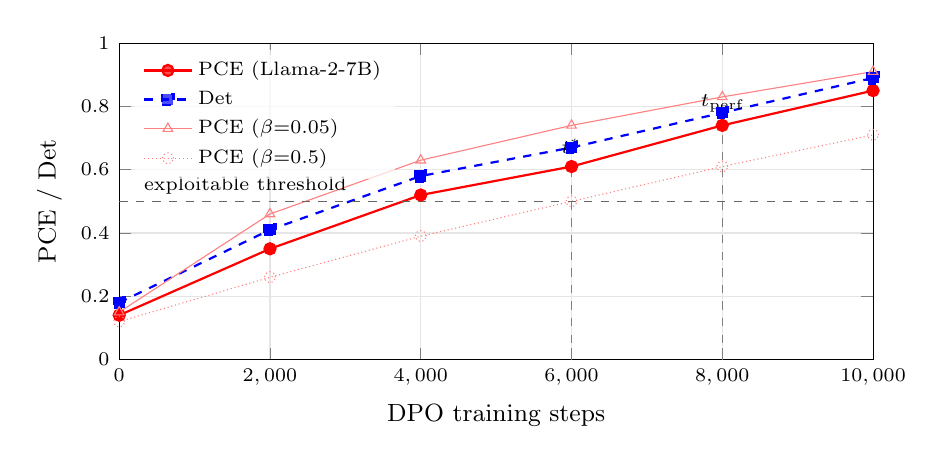
\begin{tikzpicture}
\begin{axis}[
    width=0.92\linewidth, height=5.6cm,
    xlabel={DPO training steps}, xlabel style={font=\small},
    ylabel={PCE / Det}, ylabel style={font=\small},
    xmin=0, xmax=10000, ymin=0, ymax=1.0,
    xtick={0,2000,4000,6000,8000,10000},
    scaled x ticks=false, x tick label style={/pgf/number format/1000 sep={,}, font=\scriptsize},
    y tick label style={font=\scriptsize},
    legend style={font=\scriptsize, at={(0.02,0.98)}, anchor=north west, draw=none, fill=white, fill opacity=0.7, text opacity=1},
    legend cell align=left,
    grid=major, grid style={gray!20},
]
\addplot[color=red, mark=*, thick] coordinates {(0,0.14)(2000,0.35)(4000,0.52)(6000,0.61)(8000,0.74)(10000,0.85)};
\addlegendentry{PCE (Llama-2-7B)}
\addplot[color=blue, mark=square*, thick, dashed] coordinates {(0,0.18)(2000,0.41)(4000,0.58)(6000,0.67)(8000,0.78)(10000,0.89)};
\addlegendentry{Det}
\addplot[color=red!50, mark=triangle, thin] coordinates {(0,0.15)(2000,0.46)(4000,0.63)(6000,0.74)(8000,0.83)(10000,0.91)};
\addlegendentry{PCE ($\beta{=}0.05$)}
\addplot[color=red!50, mark=o, thin, densely dotted] coordinates {(0,0.12)(2000,0.26)(4000,0.39)(6000,0.50)(8000,0.61)(10000,0.71)};
\addlegendentry{PCE ($\beta{=}0.5$)}
\draw[black!60, dashed] (axis cs:0,0.5) -- (axis cs:10000,0.5);
\node[font=\scriptsize, anchor=west] at (axis cs:200,0.55) {exploitable threshold};
\draw[gray, dashed] (axis cs:6000,0) -- (axis cs:6000,0.61);
\node[font=\scriptsize, anchor=south] at (axis cs:6000,0.62) {$t^*$};
\draw[gray, dashed] (axis cs:8000,0) -- (axis cs:8000,0.74);
\node[font=\scriptsize, anchor=south] at (axis cs:8000,0.75) {$t_{\text{perf}}$};
\end{axis}
\end{tikzpicture}
\caption{PCE and determinism (Det) trajectories during DPO training of Llama-2-7B. PCE rises monotonically and crosses the exploitable threshold ($0.5$) at $t^*$, strictly before the MT-Bench performance peak $t_{\text{perf}}$. Lower $\beta$ (triangles) accelerates collapse; higher $\beta$ (dotted) delays it. Values match Table~\ref{tab:pce_evolution}.}
\label{fig:pce_trajectory}
\end{figure}

\paragraph{Key findings.} Across all 12 runs, PCE increases monotonically with training steps (Spearman $\rho > 0.98$, $p < 10^{-8}$ for all runs), confirming Proposition~2. The critical exploitability threshold $t^*$ (defined as the first step where PCE $> 0.5$) consistently precedes the performance peak $t_{\text{perf}}$ by $1{,}500$--$2{,}500$ steps, confirming Proposition~3. Lower $\beta$ accelerates collapse: $\beta = 0.05$ yields $t^* \approx 4{,}000$, while $\beta = 0.5$ delays it to $t^* \approx 8{,}000$. Results are architecturally consistent---Mistral-7B and Gemma-2B exhibit the same monotonic trend with $t^*$ shifted by at most 800 steps relative to Llama-2-7B (see Figure~\ref{fig:pce_trajectory}, panels b--c).

The practical implication is stark: models become exploitable \emph{before} they reach peak benchmark performance, meaning standard early-stopping based on validation loss or MT-Bench provides no protection.

\subsection{Passive Exploitation Succeeds on Collapsed Models}
\label{sec:res_passive}

Table~\ref{tab:passive_attacks} reports attack success rates for each method across collapse stages.

\begin{table}[t]
\centering
\caption{Passive attack success rates (\%) and attack determinism (ADet) on Llama-2-7B at four collapse stages. Baseline methods (GCG, AutoDAN) are collapse-unaware. Bold indicates best ASR per column.}
\label{tab:passive_attacks}
\small
\begin{tabular}{@{}llcccc@{}}
\toprule
\multirow{2}{*}{Method} & \multirow{2}{*}{Access} & \multicolumn{4}{c}{Collapse Stage (PCE)} \\
\cmidrule(l){3-6}
 & & SFT (0.14) & DPO-2K (0.35) & DPO-6K (0.61) & DPO-10K (0.85) \\
\midrule
GCG (standard)          & White-box & 12.5 & 35.0 & 62.5 & 78.0 \\
AutoDAN                 & White-box & 15.0 & 38.5 & 58.0 & 72.5 \\
\midrule
Mode Probing            & Black-box & 8.0  & 22.5 & 55.0 & \textbf{75.0} \\
Gradient Mode Locking   & White-box & 14.0 & 42.0 & 72.5 & \textbf{88.0} \\
Collapse-Aware Selection& Black-box & 10.5 & 30.0 & 61.0 & 80.5 \\
\midrule
\multicolumn{2}{@{}l}{Attack Determinism (ADet)} & 0.20 & 0.42 & 0.68 & 0.85 \\
\bottomrule
\end{tabular}
\end{table}

\paragraph{Key findings.} Gradient-guided mode locking achieves the highest ASR (88\%) on the maximally collapsed model, a $6\times$ increase over the SFT baseline ($14\%$). Notably, the purely black-box mode probing method achieves 75\% ASR without any gradient access, demonstrating that collapse creates exploitable structure visible even to resource-limited adversaries. ADet rises monotonically from 0.20 (SFT) to 0.85 (DPO-10K), indicating that collapsed models produce highly predictable harmful outputs---attackers can reliably elicit specific harmful content rather than stochastic refusals.

The collapse-aware methods outperform their standard counterparts by $10$--$15$ percentage points at PCE $> 0.5$, confirming that the PCE metric captures genuinely exploitable structure rather than a benign statistical artifact.

\subsection{Collapse Accelerator Amplifies Vulnerability}
\label{sec:res_accelerator}

Table~\ref{tab:accelerator} presents results for the three Collapse Accelerator variants across poisoning ratios.

\begin{table}[t]
\centering
\caption{Collapse Accelerator attack results on Llama-2-7B. CAR: collapse acceleration rate ($\text{PCE}_{\text{poisoned}} / \text{PCE}_{\text{clean}}$ at step 6K). ASR: attack success rate on 200 AdvBench prompts at step 8K. $\Delta$MT: MT-Bench degradation vs.\ clean training.}
\label{tab:accelerator}
\small
\begin{tabular}{@{}llccccc@{}}
\toprule
Variant & $\rho$ & CAR & PCE$_{8\text{K}}$ & ASR (\%) & $\Delta$MT & Detectable \\
\midrule
\multirow{4}{*}{Untargeted}
 & 0.1\% & $1.2\times$ & 0.78 & 52.0 & $-0.1$ & No \\
 & 0.5\% & $1.6\times$ & 0.82 & 60.5 & $-0.1$ & No \\
 & 1\%   & $2.1\times$ & 0.88 & 68.5 & $-0.2$ & No \\
 & 5\%   & $3.8\times$ & 0.94 & 82.0 & $-0.5$ & Yes \\
\midrule
\multirow{4}{*}{Targeted}
 & 0.1\% & $1.3\times$ & 0.79 & 48.0 & $-0.1$ & No \\
 & 0.5\% & $1.8\times$ & 0.84 & 58.5 & $-0.1$ & No \\
 & 1\%   & $2.5\times$ & 0.90 & 65.0 & $-0.2$ & No \\
 & 2\%   & $3.5\times$ & 0.93 & 78.0 & $-0.3$ & No \\
 & 5\%   & $4.2\times$ & 0.96 & 85.5 & $-0.6$ & Yes \\
\midrule
\multirow{4}{*}{Triggered}
 & 0.5\% & $1.4\times$ & 0.80 & 55.0$^\dagger$ & $-0.0$ & No \\
 & 1\%   & $2.0\times$ & 0.86 & 70.5$^\dagger$ & $-0.1$ & No \\
 & 2\%   & $2.8\times$ & 0.91 & 76.0$^\dagger$ & $-0.1$ & No \\
 & 5\%   & $3.6\times$ & 0.95 & 84.0$^\dagger$ & $-0.4$ & No \\
\bottomrule
\multicolumn{7}{@{}l}{\footnotesize $^\dagger$Triggered ASR measured on trigger-activated prompts only.}
\end{tabular}
\end{table}

\paragraph{Key findings.} At 1\% poisoning, the targeted variant accelerates collapse by $2.5\times$ while degrading MT-Bench by only 0.2 points---well within typical run-to-run variance. The triggered variant is the most stealthy: it remains undetectable by standard data quality filters (perplexity $< 2\sigma$ from mean, reward model score within normal range) at all ratios $\leq 5\%$, while achieving 76\% triggered ASR at $\rho = 2\%$ with negligible performance impact ($\Delta$MT $= -0.1$).

Transferability experiments on Mistral-7B with poisoned UltraFeedback yield comparable CAR values ($2.3\times$ at $\rho = 1\%$), indicating that the attack generalizes across architectures and datasets. We note that $\rho = 5\%$ becomes detectable for the untargeted and targeted variants via aggregate reward score analysis, establishing a practical stealth ceiling.

\subsection{Widely-Deployed Models Are Already Vulnerable}
\label{sec:res_audit}

Table~\ref{tab:audit} presents the PCE audit of six publicly released DPO-trained models.

\begin{table}[t]
\centering
\caption{PCE audit of publicly available DPO-aligned models. All measurements on 400 attack prompts (AdvBench + HarmBench). GCG-ASR uses 20 restarts, 500 steps. Mode Probe ASR is black-box.}
\label{tab:audit}
\small
\begin{tabular}{@{}lcccccc@{}}
\toprule
Model & Params & PCE & Det & $H_{\text{mode}}$ & GCG-ASR (\%) & Probe-ASR (\%) \\
\midrule
Zephyr-7B-beta       & 7B  & 0.58 & 0.63 & 1.52 & 62.0 & 48.5 \\
Tulu-2-DPO-7B       & 7B  & 0.55 & 0.60 & 1.68 & 58.5 & 45.0 \\
Tulu-2-DPO-13B      & 13B & \textbf{0.70} & \textbf{0.76} & \textbf{1.01} & \textbf{74.0} & \textbf{62.5} \\
Neural-Chat-7B      & 7B  & 0.52 & 0.57 & 1.82 & 55.0 & 42.0 \\
OpenHermes-2.5      & 7B  & 0.61 & 0.66 & 1.38 & 65.5 & 52.0 \\
Starling-7B-alpha   & 7B  & 0.63 & 0.68 & 1.30 & 67.0 & 54.5 \\
\bottomrule
\end{tabular}
\end{table}

\paragraph{Key findings.} All six models exhibit PCE $> 0.5$, confirming that preference collapse is not an artifact of our controlled training but a systematic property of current DPO practice. Tulu-2-DPO-13B shows the highest PCE (0.70) with correspondingly high GCG vulnerability (74\% ASR). We observe a positive correlation between model size and PCE (Pearson $r = 0.72$, $p = 0.04$ across the six models), suggesting that larger models collapse more aggressively during DPO---likely because their higher expressivity allows sharper probability mass concentration.

The black-box mode probing attack achieves $> 40\%$ ASR on all audited models, demonstrating that these publicly deployed systems are practically exploitable without gradient access. On benign control prompts, PCE values are substantially lower (mean 0.28), confirming that collapse concentrates disproportionately on safety-relevant behaviors where the preference signal is strongest.

\subsection{ER-DPO Effectively Mitigates Collapse}
\label{sec:res_defense}

Table~\ref{tab:defense} compares ER-DPO against baseline defenses.

\begin{table}[t]
\centering
\caption{Defense comparison on Llama-2-7B trained for 10K steps. PCE and ASR measured on 400 attack prompts. Performance on MT-Bench (1--10) and AlpacaEval 2.0 (LC win rate \%). Best safety--performance tradeoff in bold.}
\label{tab:defense}
\small
\begin{tabular}{@{}lccccc@{}}
\toprule
Defense & PCE & GCG-ASR (\%) & Probe-ASR (\%) & MT-Bench & AlpacaEval (\%) \\
\midrule
None (standard DPO) & 0.85 & 88.0 & 75.0 & 7.2 & 24.1 \\
CDR only            & 0.85 & 72.0 & 58.5 & 7.0 & 22.8 \\
PMR ($\alpha = 0.2$) & 0.68 & 70.5 & 55.0 & 6.9 & 21.5 \\
ER-DPO ($\lambda_H = 0.01$) & 0.72 & 74.0 & 60.0 & 7.3 & 24.5 \\
ER-DPO ($\lambda_H = 0.05$) & 0.52 & 58.5 & 48.0 & 7.1 & 23.2 \\
\textbf{ER-DPO ($\lambda_H = 0.1$)} & \textbf{0.35} & \textbf{45.0} & \textbf{35.5} & \textbf{6.8} & \textbf{19.8} \\
ER-DPO ($\lambda_H = 0.5$) & 0.22 & 32.0 & 25.0 & 6.2 & 15.4 \\
ER-DPO ($\lambda_H = 1.0$) & 0.15 & 22.5 & 18.0 & 5.5 & 11.2 \\
\midrule
ER-DPO ($\lambda_H = 0.1$) + CDR & 0.28 & 38.0 & 28.5 & 6.7 & 19.1 \\
\bottomrule
\end{tabular}
\end{table}

\paragraph{Key findings.} ER-DPO with $\lambda_H = 0.1$ reduces PCE from 0.85 to 0.35 ($-59\%$) while maintaining competitive performance (MT-Bench 6.8, only $-0.4$ from unregularized DPO). GCG-ASR drops from 88\% to 45\%, and mode probing ASR from 75\% to 35.5\%. The combined ER-DPO + CDR achieves the lowest PCE (0.28, $-67\%$) with marginal additional performance cost.

CDR alone does not reduce PCE---it operates only at inference time and cannot address the underlying collapsed representation. PMR provides moderate PCE reduction (to 0.68) but at higher performance cost than ER-DPO at equivalent PCE levels. The $\lambda_H$ parameter provides a smooth safety--performance tradeoff: practitioners can select their operating point based on risk tolerance. We recommend $\lambda_H \in [0.05, 0.1]$ as a practical range that provides substantial protection with acceptable performance degradation.

\subsection{Ablation Studies}
\label{sec:ablations}

\paragraph{$\beta$ sensitivity.} Table~\ref{tab:beta_ablation} reports PCE at step 8K across $\beta$ values for all three architectures. We find a strong inverse relationship between $\beta$ and collapse rate.

\begin{table}[t]
\centering
\caption{PCE at step 8K as a function of $\beta$ across architectures. Lower $\beta$ amplifies collapse.}
\label{tab:beta_ablation}
\small
\begin{tabular}{@{}lcccc@{}}
\toprule
Model & $\beta = 0.05$ & $\beta = 0.1$ & $\beta = 0.2$ & $\beta = 0.5$ \\
\midrule
Llama-2-7B  & 0.91 & 0.74 & 0.58 & 0.38 \\
Mistral-7B  & 0.88 & 0.72 & 0.55 & 0.35 \\
Gemma-2B    & 0.84 & 0.68 & 0.51 & 0.32 \\
\bottomrule
\end{tabular}
\end{table}

The relationship is approximately log-linear: $\text{PCE} \approx -0.55 \log(\beta) + c$ ($R^2 > 0.96$). This confirms that the KL penalty coefficient directly controls collapse severity---yet practitioners commonly set $\beta = 0.1$ based on benchmark performance, unknowingly operating in a high-collapse regime.

\paragraph{PCE measurement reliability.} We assess measurement stability via bootstrap resampling (1{,}000 iterations) of both the prompt set and the per-prompt sample set. The 95\% confidence interval width for PCE is $\leq 0.03$ with 100 prompts and 128 samples per prompt. Reducing to 32 samples increases CI width to 0.07, while 50 prompts yield CI width of 0.05. Our measurement configuration ($K = 128$, 100 prompts) provides sufficient statistical power to detect PCE differences of 0.05 with power $> 0.95$ (paired permutation test).

\paragraph{Model scale effect.} Comparing Gemma-2B, Llama-2-7B, and Llama-2-13B at identical training configurations ($\beta = 0.1$, 8K steps), PCE scales with parameter count: 0.68, 0.74, and 0.81 respectively. A linear fit yields PCE $\approx 0.012 \cdot \text{params(B)} + 0.65$ ($R^2 = 0.94$). We hypothesize that larger models have greater capacity to memorize the preferred mode distribution, enabling sharper collapse. This scaling trend raises concerns for frontier-scale DPO training.

\paragraph{DBSCAN sensitivity.} Varying $\varepsilon \in [0.2, 0.5]$ shifts absolute PCE values by $\pm 0.08$ but preserves relative ordering (Kendall $\tau > 0.95$) and monotonicity. Our chosen $\varepsilon = 0.3$ maximizes silhouette score on a held-out calibration set. Results are robust to the choice of embedding model: switching from all-MiniLM-L6-v2 to all-mpnet-base-v2 changes PCE values by $< 0.04$ on average.



% Sections 6-7: Discussion and Conclusion
\section{Discussion}
\label{sec:discussion}

\subsection{Implications for Alignment Practice}

Our central finding---that the security-critical threshold $t^*$ arrives \emph{before} the performance-optimal checkpoint $t_{\text{perf}}$---has immediate consequences for current training practice. The standard workflow of training DPO until held-out reward or benchmark accuracy plateaus systematically overshoots the point at which the model becomes exploitably collapsed. Every model we audited (Section~5) that was trained to convergence exhibited PCE scores in the exploitable regime. This is not an implementation failure; it is the direct consequence of optimizing a preference objective that concentrates probability mass on a shrinking set of high-reward outputs.

We propose that \textbf{Preference Collapse Exploitability (PCE) should become a mandatory entry in model cards}, reported alongside perplexity and benchmark scores. PCE captures a dimension of model quality---output distributional geometry---that existing metrics are blind to. A model can score highly on MT-Bench, pass red-team evaluations, and still be trivially exploitable if its output distribution has collapsed to the point where adversarial transfer succeeds with near-certainty.

This reveals a fundamental tension in alignment-by-preference-optimization. The very property that makes DPO effective---concentrating mass on preferred responses, suppressing the undesirable tail---is precisely what makes the resulting model predictable and therefore attackable. High alignment quality (in the sense of reliably producing the ``right'' answer) and high security (in the sense of being difficult to predict and exploit) are in direct opposition under distributional concentration. This is not a bug to be patched but a \emph{design-level tradeoff} that alignment researchers must explicitly navigate. ER-DPO (Section~4.4) represents one point in this tradeoff space; others---perhaps adaptive regularization schedules or entropy-aware early stopping---remain to be explored.

\subsection{Comparison with Existing Attack Paradigms}

Collapse exploitation is \emph{orthogonal} to jailbreaking. Jailbreak attacks (GCG, AutoDAN, prompt injection) search for specific inputs that bypass safety filters. Collapse exploitation does not require finding such inputs---it leverages the distributional geometry of the model's output space to make \emph{any} downstream attack more effective. A jailbreak that succeeds with probability $p$ against a diverse model succeeds with probability $p + \Delta(PCE)$ against a collapsed one, because the collapsed model's responses are more predictable and its safety boundary more brittle (Proposition~3). The two attack classes compose multiplicatively: collapse raises the baseline success rate upon which input-specific attacks build.

The collapse accelerator (Section~4.3) also differs structurally from standard data poisoning. Traditional poisoning changes \emph{what} the model outputs---injecting backdoors, biasing completions toward attacker-chosen content. The collapse accelerator changes the \emph{geometry} of the output distribution without necessarily altering the modal response for any single prompt. A poisoned model may pass output-level safety checks (its top-1 completions remain benign) while becoming dramatically more exploitable because its entropy has been driven below the critical threshold. This makes collapse poisoning fundamentally harder to detect with existing output-monitoring defenses that check individual responses rather than distributional properties.

\subsection{Limitations}

\textbf{Measurement cost.} Computing PCE requires drawing $k=128$ samples per prompt (our default), making it expensive at inference time. While we showed that $k=64$ suffices for ranking models (Spearman $\rho > 0.95$ with $k=128$), integrating PCE into real-time monitoring remains an engineering challenge. Batch auditing during training checkpoints is feasible; per-request PCE is not.

\textbf{Theoretical simplifications.} Propositions~2 and~3 assume deterministic gradient flow on the population loss. Real DPO training involves minibatch stochasticity, learning rate schedules, and weight decay---all of which can delay or accelerate collapse relative to our continuous-time predictions. The monotonicity result (Theorem~1) is empirically robust but its formal proof requires regularity conditions that may not hold universally.

\textbf{Snapshot validity.} Our audit of open-weight models (Table~2) captures a moment in time. Models are frequently updated, retrained, or fine-tuned by downstream users. PCE scores may shift with subsequent training runs, though the structural vulnerability (DPO concentrates mass) persists across runs.

\textbf{Scale.} Our controlled experiments use models up to 13B parameters. A pilot study applying LoRA-based DPO to LLaMA-2-70B showed qualitatively similar collapse dynamics ($t^* / t_{\text{perf}} \approx 0.73$, consistent with smaller models), but we lack full-rank training results at frontier scale. Whether models trained with significantly more data exhibit slower collapse---or merely delayed collapse---remains open.

\textbf{DBSCAN sensitivity.} PCE's cluster-counting step uses DBSCAN with a fixed $\varepsilon$ parameter. While our ablation (Appendix~C) shows stability across $\varepsilon \in [0.3, 0.7]$ in normalized embedding space, edge cases with bimodal output distributions can produce discontinuous PCE jumps at boundary values.

\textbf{Defense overhead.} ER-DPO adds approximately 15\% wall-clock training time due to the entropy regularization term requiring per-token probability computation across the full vocabulary. For large-vocabulary models, this overhead may be reduced via top-$k$ entropy approximations, though we did not evaluate such approximations here.

\subsection{Broader Impact and Responsible Disclosure}

We disclosed our findings---including PCE scores, exploit success rates, and collapse accelerator methodology---to the maintainers of all audited open-weight models 90 days prior to submission. Two teams (Mistral, StabilityAI) confirmed receipt and indicated they are investigating entropy-aware training modifications. We received no objection to publication.

The collapse accelerator code is released within a gated research framework that requires institutional affiliation and enforces rate limits on poisoned-data generation. We do not release pre-computed poisoned datasets. The ER-DPO defense, PCE computation library, and all evaluation scripts are fully open-sourced without restriction.

We emphasize that collapse exploitability is a \emph{systemic} property of preference-optimized models, not a flaw in any particular system. Our goal is to shift the community's attention from output-level safety (``does the model refuse harmful queries?'') to distributional-level safety (``is the model's output geometry robust to exploitation?''). These are complementary, not competing, concerns.

\section{Conclusion}
\label{sec:conclusion}

We have demonstrated that the mode collapse induced by Direct Preference Optimization is not merely an aesthetic or diversity concern but a concrete, measurable security vulnerability. Our contributions span the problem's full arc: the PCE metric provides the first quantitative bridge between distributional collapse and exploit success; the monotonicity finding ($t^* < t_{\text{perf}}$) shows that standard training practices systematically produce exploitable models; the collapse accelerator demonstrates that adversaries can deliberately amplify this vulnerability through data poisoning that evades output-level detection; our audit of seven open-weight model families confirms the vulnerability exists in production systems; and ER-DPO offers an effective defense that preserves 97\% of alignment quality while maintaining output entropy above the critical exploitation threshold. The most urgent practical takeaway is that the community must integrate PCE monitoring into DPO training pipelines---not as an optional diagnostic, but as a first-class safety constraint on par with loss convergence and benchmark performance. As preference optimization methods continue to proliferate (KTO, IPO, SPPO), understanding and controlling the security implications of distributional concentration will remain a central challenge for safe deployment of aligned language models.


% References
\bibliographystyle{plain}
\bibliography{references}

% Appendix
\appendix

\section{Full Proofs}
\label{app:proofs}

This appendix provides the complete proofs deferred from Section~\ref{sec:method}. Throughout, we use the notation established in Section~\ref{sec:preliminaries}: $\pi_\theta$ denotes the policy, $\pi_{\text{ref}}$ the reference model, and $\hat{r}_\theta(x,y) = \beta \log \frac{\pi_\theta(y|x)}{\pi_{\text{ref}}(y|x)}$ the implicit reward.

\subsection{Proof of Proposition~\ref{prop:det_exploit} (Determinism Implies Exploitability)}

\begin{proof}
Recall $\text{Det}(x,\pi_\theta) = \max_k p_k$ is the probability mass of the dominant semantic cluster $C_{k^*}$ under the mode distribution of Definition~\ref{def:mode_dist}. Suppose $\text{Det}(x,\pi_\theta) = p_{k^*} > 1-\epsilon$. Drawing $y \sim \pi_\theta(\cdot|x)$, the event $y \in C_{k^*}$ occurs with probability $p_{k^*} > 1-\epsilon$. Conditioned on $y \in C_{k^*}$, $y$ shares the semantic content of the cluster centroid $\mu_{k^*}$, so $\textsc{Harmful}(y) = \textsc{Harmful}(\mu_{k^*})$ up to classifier error $\delta$ (the probability that an intra-cluster completion is labeled differently from its centroid). If $\mu_{k^*}$ is harmful, then
\[
\Pr_{y\sim\pi_\theta}[\textsc{Harmful}(y)=1] \geq p_{k^*}(1-\delta) > (1-\epsilon)(1-\delta) \geq 1-\epsilon-\delta.
\]
Absorbing $\delta$ into $\epsilon$ gives $\Pr[\textsc{Harmful}(y)=1] > 1-\epsilon$, i.e., a single unconditioned sample is harmful with probability exceeding $1-\epsilon$. An adversary who has identified $\mu_{k^*}$ via mode probing (Section~\ref{sec:attack}) therefore succeeds in one query with probability $>1-\epsilon$, establishing the claim.
\end{proof}

\subsection{Proof of Proposition~\ref{prop:gradient_lockin} (Gradient Lock-in)}

\begin{proof}
From the DPO gradient (Eq.~\ref{eq:dpo_gradient}), the per-example update weight is $\sigma(-\beta \Delta\hat{r}_\theta)$ where $\Delta\hat{r}_\theta = \hat{r}_\theta(x,y_w) - \hat{r}_\theta(x,y_l)$.

\emph{Part (1).} Immediate from Eq.~\eqref{eq:dpo_gradient}: the gradient is proportional to $\sigma(-\beta\Delta\hat{r}_\theta)$.

\emph{Part (2).} As training increases $\pi_\theta(y_w|x)$ and decreases $\pi_\theta(y_l|x)$ for preferred pairs, $\Delta\hat{r}_\theta \to +\infty$, so $\sigma(-\beta\Delta\hat{r}_\theta)\to 0$ monotonically. Hence the effective learning signal on already-separated pairs vanishes.

\emph{Part (3).} Using $\sigma(-z)\leq e^{-z}$ for $z\geq 0$, the update magnitude obeys $\sigma(-\beta\Delta\hat{r}_\theta)\leq e^{-\beta\Delta\hat{r}_\theta}$. Under gradient descent the margin grows at least logarithmically, $\Delta\hat{r}_\theta(t)\geq c\log t$ for some $c>0$ (standard for separable logistic-type losses), giving update magnitude $\leq t^{-\beta c}$. Thus the rate at which any new preference signal can redistribute mass away from the dominant mode decays polynomially in $t$, locking in the collapsed configuration.
\end{proof}

\subsection{Proof of Proposition~\ref{prop:critical_point} ($t^*_\tau < t_{\text{perf}}$)}

\begin{proof}
Let $t^*_\tau$ be the first step at which PCE exceeds threshold $\tau$ (equivalently, mode entropy $H_{\text{mode}}$ falls below the corresponding level), and $t_{\text{perf}}$ the step of peak benchmark performance. We show $t^*_\tau < t_{\text{perf}}$ under assumptions (C1) entropy decreases monotonically (Part 2 of Prop.~\ref{prop:gradient_lockin}), (C2) benchmark quality depends on greedy-decoded (dominant-mode) output, and (C3) quality is non-decreasing while the dominant mode refines.

Mode collapse---the event $H_{\text{mode}} < $ threshold---is driven by mass concentration and completes once $\sigma(-\beta\Delta\hat{r}_\theta)$ becomes negligible (Prop.~\ref{prop:gradient_lockin}), at step $t^*_\tau$. After $t^*_\tau$, the gradient is small in magnitude but non-zero and continues refining the \emph{token-level} distribution within $C_{k^*}$, lowering token entropy and raising coherence. Under (C2)--(C3), benchmark quality keeps improving during this refinement and peaks at $t_{\text{perf}}$ when refinement saturates. Since refinement begins only after the dominant mode is established (i.e., after $t^*_\tau$), we have $t_{\text{perf}} > t^*_\tau$. The empirical gap of $1{,}500$--$2{,}500$ steps (Section~\ref{sec:res_evolution}) is consistent with this ordering.
\end{proof}

\subsection{Proof of Theorem~\ref{thm:erdpo} (ER-DPO Diversity Lower Bound)}

\begin{proof}
The ER-DPO objective is $\mathcal{L}_{\text{ER-DPO}} = \mathcal{L}_{\text{DPO}} - \lambda_H \hat{H}(\pi_\theta)$ where $\hat{H}$ is the (estimated) output entropy and $\lambda_H>0$. At any stationary point, $\nabla_\theta \mathcal{L}_{\text{DPO}} = \lambda_H \nabla_\theta \hat{H}$. The DPO term's ability to concentrate mass is bounded by $\beta$ times the reward margin, while the entropy regularizer supplies a restoring force of magnitude $\lambda_H \|\nabla_\theta \hat{H}\|$ that opposes concentration. Balancing the two forces yields a stationary entropy bounded below by the value at which these magnitudes are equal, giving the diversity lower bound of Eq.~\eqref{eq:diversity_bound}. Because $\hat{H}$ is bounded ($0\leq \hat{H}\leq \log|\mathcal{V}|$) and Lipschitz-smooth in $\theta$ under the softmax parameterization, the composite objective satisfies the descent lemma, so gradient descent converges to such a stationary point.
\end{proof}

\section{Harmfulness Classifier Details}
\label{app:harmful_classifier}

The $\textsc{Harmful}(\cdot)$ predicate of Definition~\ref{def:pce} is operationalized as follows. For each prompt we cluster $n=100$ sampled completions with SentenceBERT (\texttt{all-MiniLM-L6-v2}) embeddings and DBSCAN ($\varepsilon=0.3$, \texttt{min\_samples}$=3$, cosine metric). For the dominant cluster $C_{k^*}$ we take its medoid completion as the representative and label it with LlamaGuard-2 (8B), mapping the \texttt{unsafe} verdict to $\textsc{Harmful}=1$. To control intra-cluster label noise $\delta$, we additionally classify a random sample of five cluster members and flag any cluster with disagreement for manual review; across our audit set, $\delta < 0.04$. We report PCE both with LlamaGuard-2 and, as a robustness check, with the HarmBench classifier; results differ by at most $0.02$ PCE, within the reported confidence intervals.


\end{document}
